\begin{enunciado}
 En el plano af\'{\i}n se consideran dos tri\'angulos $ABC$ y $A'B'C'$
 tales que las tres rectas $AA'$, $BB'$ y $CC'$ pasan por un mismo punto
 $O$.
 Sean $P$, $Q$ y $R$ los puntos de intersecci\'on
 de los siguientes pares de rectas:
 $AB$ y $A'B'$, $BC$ y $B'C'$ y $CA$ y $C'A'$.
 Compru\'ebese que los puntos $P$, $Q$ y $R$ est\'an alineados
 (teorema de Desargues).
\end{enunciado}

\begin{solucion}
 Se considera la referencia cartesiana con origen en $O$:
 $(O;\bar{e}_1,\bar{e}_2)$, de modo que $\bar{e}_1$ tenga la direcci\'on
 de $OA$ y $\bar{e}_2$ tenga la direcci\'on $OB$,
 y que $C$ tenga la coordenada $(1,1)$.
 Esto se puede hacer considerando los vectores $\bar{e}_1$ y $\bar{e}_2$
 con origne en $O$ y punto final en $O+r_1(A-O)$ y $O+r_2(B-O)$,
 respectivamente, donde $r_1$ es la distancia del segmento $OC$
 entre la distancia del segmento $OA$
 y $r_2$ es la distancia del segmento $OC$
 entre la distancia del segmento $OB$.
 Adem\'as, al estar $A'$, $B'$ y $C'$ sobre la misma recta
 que $OA$, $OB$ y $OC$, respectivamente,
 entonces las coordenadas se pueden resumir como sigue:
 \begin{eqnarray*}
  O(0,0) & \hspace{5cm} & \\
  A(h,0) & & A'(h',0) \\
  B(0,k) & & B'(0,k') \\
  C(1,1) & & C'(r,r)
 \end{eqnarray*}
 Entonces, por la ecuaci\'on can\'onica (o segmentada),
 se tiene que las rectas $AB$ y $A'B'$ tienen las siguientes f\'ormulas:
 \begin{eqnarray*}
  AB: & \frac{x}{h} + \frac{y}{k} = 1 & \Leftrightarrow kx+hy = hk \\
  A'B': & \frac{x}{h'} + \frac{y}{k'} = 1 & \Leftrightarrow k'x+h'y = h'k'
 \end{eqnarray*}
 Entonces $P$, el punto de intersecci\'on de $AB$ con $A'B'$, se calcula
 como sigue,
 obteniendo primera la coordenada $x$ como se muestra a continuaci\'on:
 \begin{eqnarray*}
  \begin{tabular}{c|ccccc}
   $h'$ & $kx$  & $+$ & $hy$  & $=$ & $hk$   \\
   $-h$ & $k'x$ & $+$ & $h'y$ & $=$ & $h'k'$ \\
   \hline 
   & $\left(h'k-hk'\right)x$ & & & $=$ & $hh'k-hh'k'$
  \end{tabular}
  & \Rightarrow &
  x = \frac{hh'\left( k-k' \right)}{h'k-hk'}
 \end{eqnarray*}
 An\'alogamente, la segunda coordenada se calcula como sigue:
 \begin{eqnarray*}
  \begin{tabular}{c|ccccc}
   $-k'$ & $kx$  & $+$ & $hy$  & $=$ & $hk$   \\
   $k$   & $k'x$ & $+$ & $h'y$ & $=$ & $h'k'$ \\
   \hline 
   & & & $\left( h'k-hk' \right)y$ & $=$ & $h'kk'-hkk'$
  \end{tabular}
  & \Rightarrow &
  y = \frac{kk'\left( h' - h \right)}{h'k-hk'}
 \end{eqnarray*}
 Luego, las rectas $BC$ y $B'C'$ se pueden calcular
 usando la ecuaci\'on de una recta que pasa por dos puntos, como sigue:
 \begin{eqnarray*}
  BC: & & x = \frac{y-k}{1-k} \\
  B'C': & & \frac{x}{r} = \frac{y-k'}{r-k'}
 \end{eqnarray*}
 Entonces, $Q$, el punto de intersecci\'on de $BC$ con $B'C'$,
 se calcula como sigue, obteniendo primero la segunda coordenada
 por igualaci\'on de la primera coordenada. Esto es:
 \begin{eqnarray*}
  \frac{y-k}{1-k} = \frac{r(y-k')}{r-k'} & \Leftrightarrow &
  (y-k)(r-k') = (ry-rk')(1-k) \\
  & \Leftrightarrow &
  y(r-k') - y(r-kr) = kr - kk' -rk' + kk'r \\
  & \Leftrightarrow &
  y\left( \cancel{r} - k'- \cancel{r} + kr\right) = 
  r\left(k-k'\right) + kk'(r-1) \\
  & \Leftrightarrow & y = \frac{r\left(k-k'\right) + kk'(r-1)}{kr-k'}
 \end{eqnarray*}
 y, por lo tanto, la primera coordenada se calcula como sigue:
 \begin{eqnarray*}
  x & = & 
  \frac{\left(\frac{r\left(k-k'\right)+kk'(r-1)}{kr-k'}\right) - k}{1-k} 
  = \frac{kr-k'r+kk'r-kk'-k\left( kr-k'\right)}{\left(kr-k'\right)(1-k)} \\
  & = &
  \frac{kr-k'r+kk'r-\cancel{kk'}-k^2r+\cancel{kk'}}{\left(kr-k'\right)(1-k)}
  = \frac{kr(1-k)-k'r(1-k)}{\left(kr-k'\right)(1-k)} \\
  & = & 
  \frac{r\left(k-k'\right)\cancel{(1-k)}}{\left(kr-k'\right)\cancel{(1-k)}}
  = \frac{r\left(k-k'\right)}{kr-k'}
 \end{eqnarray*}
 Y, las rectas $CA$ y $C'A'$ se pueden calcular usando la ecuaci\'on
 de una recta que pasa por dos puntos, como sigue:
 \begin{eqnarray*}
  CA: & & \frac{x-h}{1-h} = y \\
  C'A': & & \frac{x-h'}{r-h'} = \frac{y}{r}
 \end{eqnarray*}
 Entonces, $R$, el punto de intersecci\'on de $CA$ y $C'A'$,
 se calcula como sigue, obteniendo primero la coordenada $x$
 por igualaci\'on de la segunda coordenada. Esto es:
 \begin{eqnarray*}
  \frac{x-h}{1-h} = \frac{r\left(x-h'\right)}{r-h'} & \Leftrightarrow & 
  \left( r-h' \right)(x-h) = \left( rx-h'r \right)(1-h) \\
  & \Leftrightarrow &
  \left( r-h' \right)x - r(1-h)x = h\left( r-h' \right) - h'r(1-h) \\
  & \Leftrightarrow &
  \left( \cancel{r} - h' - \cancel{r} + hr \right) =
  hr-hh'-h'r + hh'r \\
  & \Leftrightarrow & 
  x = \frac{r\left( h - h' \right) + hh'(r-1)}{hr-h'}
 \end{eqnarray*}
 y, por lo tanto, la segunda coordenada se calcula como sigue
 \begin{eqnarray*}
  y & = & 
  \frac{\left(\frac{r\left(h-h'\right) + hh'(r-1)}{hr-h'}\right)-h}{1-h} 
  = \frac{hr-h'r+hh'r-hh'-h\left(hr-h'\right)}{\left(hr-h'\right)(1-h)}
  \\ & = & 
  \frac{hr-h'r+hh'r-\cancel{hh'}-h^2r+\cancel{hh'}}{\left(hr-h'\right)(1-h)}
  = \frac{hr(1-h)-h'r(1-h)}{\left(hr-h'\right)(1-h)} \\
  & = & 
  \frac{r\left(h-h'\right)\cancel{(1-h)}}{\left(hr-h'\right)\cancel{(1-h)}}
  = \frac{r\left(h-h'\right)}{hr-h'}
 \end{eqnarray*}
 En resumen, las coordenada de los puntos $P$, $Q$ y $R$ son:
 \begin{eqnarray*}
  P & = & \left( x_P, y_P \right) =
  \left( \frac{hh'\left( k-k' \right)}{h'k-hk'}, 
  \frac{kk'\left( h'-h \right)}{h'k-hk'} \right) \\
  Q & = & \left( x_Q, y_Q \right) =
  \left( \frac{r\left( k-k' \right)}{kr-k'}, 
  \frac{r\left( k-k' \right) + kk'(r-1)}{kr-k'} \right) \\
  R & = & \left( x_R, y_R \right) =
  \left( \frac{r\left( h - h' \right) + hh'(r-1)}{hr-h'},
  \frac{r\left(h-h'\right)}{hr-h'} \right)
 \end{eqnarray*}
 Entonces la direcci\'on de la recta $QR$ est\'a dado
 por la direcci\'on del vector
 $\overrightarrow{QR} = \left( x_R-x_Q, y_R-y_Q \right)$ 
 y la direcci\'on de la recta $QP$ est\'a dado
 por la direcci\'on del vector
 $\overrightarrow{QP} = \left( x_P-x_Q, y_P-y_Q \right)$,
 entonces las rectas $QR$ y $QP$ son iguales si y s\'olo si son paralelas,
 pues si son paralelas, entonces pertenecen a la misma familia de paralelas
 pero s\'olo hay una \'unica recta de una familia de paralelas que pasa
 por un punto dado, en este caso $Q$.
 Luego entonces, las rectas $QR$ y $QP$ son paralelas
 si y s\'olo si los vectores
 $\overrightarrow{QR}$ y $\overrightarrow{QP}$ son proporcionales
 si y s\'olo si $\frac{x_R-x_Q}{x_P-x_Q} = \frac{y_R-y_Q}{y_P-y_Q}$
 si y s\'olo si $\frac{y_R-y_Q}{x_R-x_Q} = \frac{y_P-y_P}{x_P-x_Q}$,
 luego, como ambas coordenadas de un punto tienen los mismos denominadores
 digamos,
 $P=\left( x_P, y_P \right) = \left( \frac{a}{c},\frac{b}{c} \right)$,
 $Q=\left( x_Q, y_Q \right) = \left( \frac{a'}{c'},\frac{b'}{c'} \right)$ y
 $R=\left( x_R,y_R\right) =\left( \frac{a''}{c''},\frac{b''}{c''} \right)$,
 entonces $\frac{y_P-y_Q}{x_P-x_Q} = \frac{b/c-b'/c'}{a/c-a'/c'}
 = \frac{\frac{bc'-b'c}{cc'}}{\frac{ac'-a'c}{cc'}}
 = \frac{bc'-b'c}{ac'-a'c}$
 y, an\'alogamente,
 $\frac{y_R-y_Q}{x_R-x_Q} = \frac{b''c'-b'c''}{a''c'-a'c''}$.
 Luego entonces, al hacer los c\'alculos se tiene que:
 \begin{eqnarray*}
  b''c'-b'c'' & = &
  r\left( h-h' \right)\left( kr - k' \right) -
  \left[ r\left( k-k' \right) + kk'(r-1) \right]\left( hr-h' \right) \\
  & = & r\left[ \left( h-h' \right)\left( kr-k' \right) -
  \left( k-k' \right)\left( hr-h' \right) \right] -
  kk'(r-1)\left( hr - h' \right) \\
  & = & r\left( \cancel{hkr} - hk' - h'kr + \cancel{h'k'} - \cancel{hkr} + h'k + hk'r - \cancel{h'k'} \right)
  - kk'(r-1)\left( hr - h' \right) \\
  & = & r\left( hk'r - h'kr - hk' + h'k  \right) 
  - kk'(r-1)\left( hr - h' \right) \\
  & = & r\left[ (r-1)\left( hk' - h'k \right) \right]
  - kk'(r-1)\left( hr - h' \right) \\
  & = & (r-1)\left[ r\left( hk'-h'k\right)-kk'\left( hr-h'\right)\right] \\
  a''c'-a'c'' & = &
  \left[ r\left( h-h' \right) + hh'(r-1) \right]\left( kr-k' \right) - 
  r\left( k-k' \right)\left( hr - h' \right) \\
  & = & r \left[ \left( h-h' \right)\left( kr-k' \right) - 
  \left( k-k' \right)\left( hr - h' \right) \right] +
  hh'(r-1)\left( kr - k' \right) \\
  & = & r\left[ (r-1)\left( hk' - h'k \right) \right] +
  hh'(r-1)\left( kr - k' \right) \\
  & = & (r-1)\left[r\left( hk'-h'k\right)+hh'\left( kr-k'\right)\right]
 \end{eqnarray*}
 Entonces
 \begin{equation*}
  \frac{y_R-y_Q}{x_R-x_Q} =
  \frac{\cancel{(r-1)}\left[ r\left( hk'-h'k\right)-kk'\left( hr-h'\right)\right]
  }{
  \cancel{(r-1)}\left[r\left( hk'-h'k\right)+hh'\left( kr-k'\right)\right]
  }
  =
  \frac{r\left( hk'-h'k\right)-kk'\left( hr-h'\right)}{r\left( hk'-h'k\right)+hh'\left( kr-k'\right)}
 \end{equation*}
 Por otro lado, se tiene que:
 \begin{eqnarray*}
  bc'-b'c & = &
  kk'\left( h'-h \right)\left( kr-k' \right) -
  \left[ r\left( k-k'\right) + kk'(r-1) \right]\left( h'k-hk' \right) \\
  & = & kk'\left[ \left( h'-h \right)\left( kr-k' \right) -
  (r-1)\left( h'k-hk' \right) \right] -
  r\left( k - k' \right)\left( h'k - hk' \right) \\
  & = & kk'\left( \cancel{h'kr} - h'k' - hkr + \cancel{hk'} - \cancel{h'kr} + hk'r + h'k - \cancel{hk'} \right)
  - r\left( k - k' \right)\left( h'k - hk' \right) \\
  & = & kk'\left( h'k - h'k' + hk'r - hkr \right) + 
  r\left( hk' - h'k \right)\left( k - k' \right) \\
  & = & kk'\left( h' - hr \right)\left( k-k'\right) +
  r\left( hk' - h'k \right)\left( k - k' \right) \\
  & = & \left( k - k' \right)\left[ r\left( hk' - h'k \right) - kk'\left( hr - h' \right) \right] \\
  ac' - a'c & = &
  hh'\left( k - k' \right)\left( kr - k' \right) - 
  r\left( k - k' \right)\left( h'k - hk' \right) \\
  & = &
  \left( k - k' \right)\left[ r\left( hk' - h'k \right) + 
  hh'\left( kr - k' \right) \right]
 \end{eqnarray*}
 Entonces
 \begin{equation*}
  \frac{y_P - y_Q}{x_P - x_Q} = 
  \frac{
  \cancel{\left( k - k' \right)}
  \left[ r\left( hk' - h'k \right) - kk'\left( hr - h' \right) \right]
  }{
  \cancel{\left( k - k' \right)}
  \left[ r\left( hk' - h'k \right) + hh'\left( kr - k' \right) \right]
  }
  =
  \frac{
  r\left( hk' - h'k \right) - kk'\left( hr - h' \right)
  }{
  r\left( hk' - h'k \right) + hh'\left( kr - k' \right)
  }
 \end{equation*}
 Por lo tanto,
 como $\frac{y_R - y_Q}{x_R - x_Q} = \frac{y_P - y_Q}{x_P - x_Q}$, 
 se concluye que las rectas $QR$ y $QP$ son paralelas
 y, como pasan por el mismo punto $Q$, por lo tanto, son iguales.
 Por lo tanto, los puntos $P$, $Q$ y $R$ est\'an alineados.
 Q.E.D.${}_{\blacksquare}$
 
 \begin{center}
  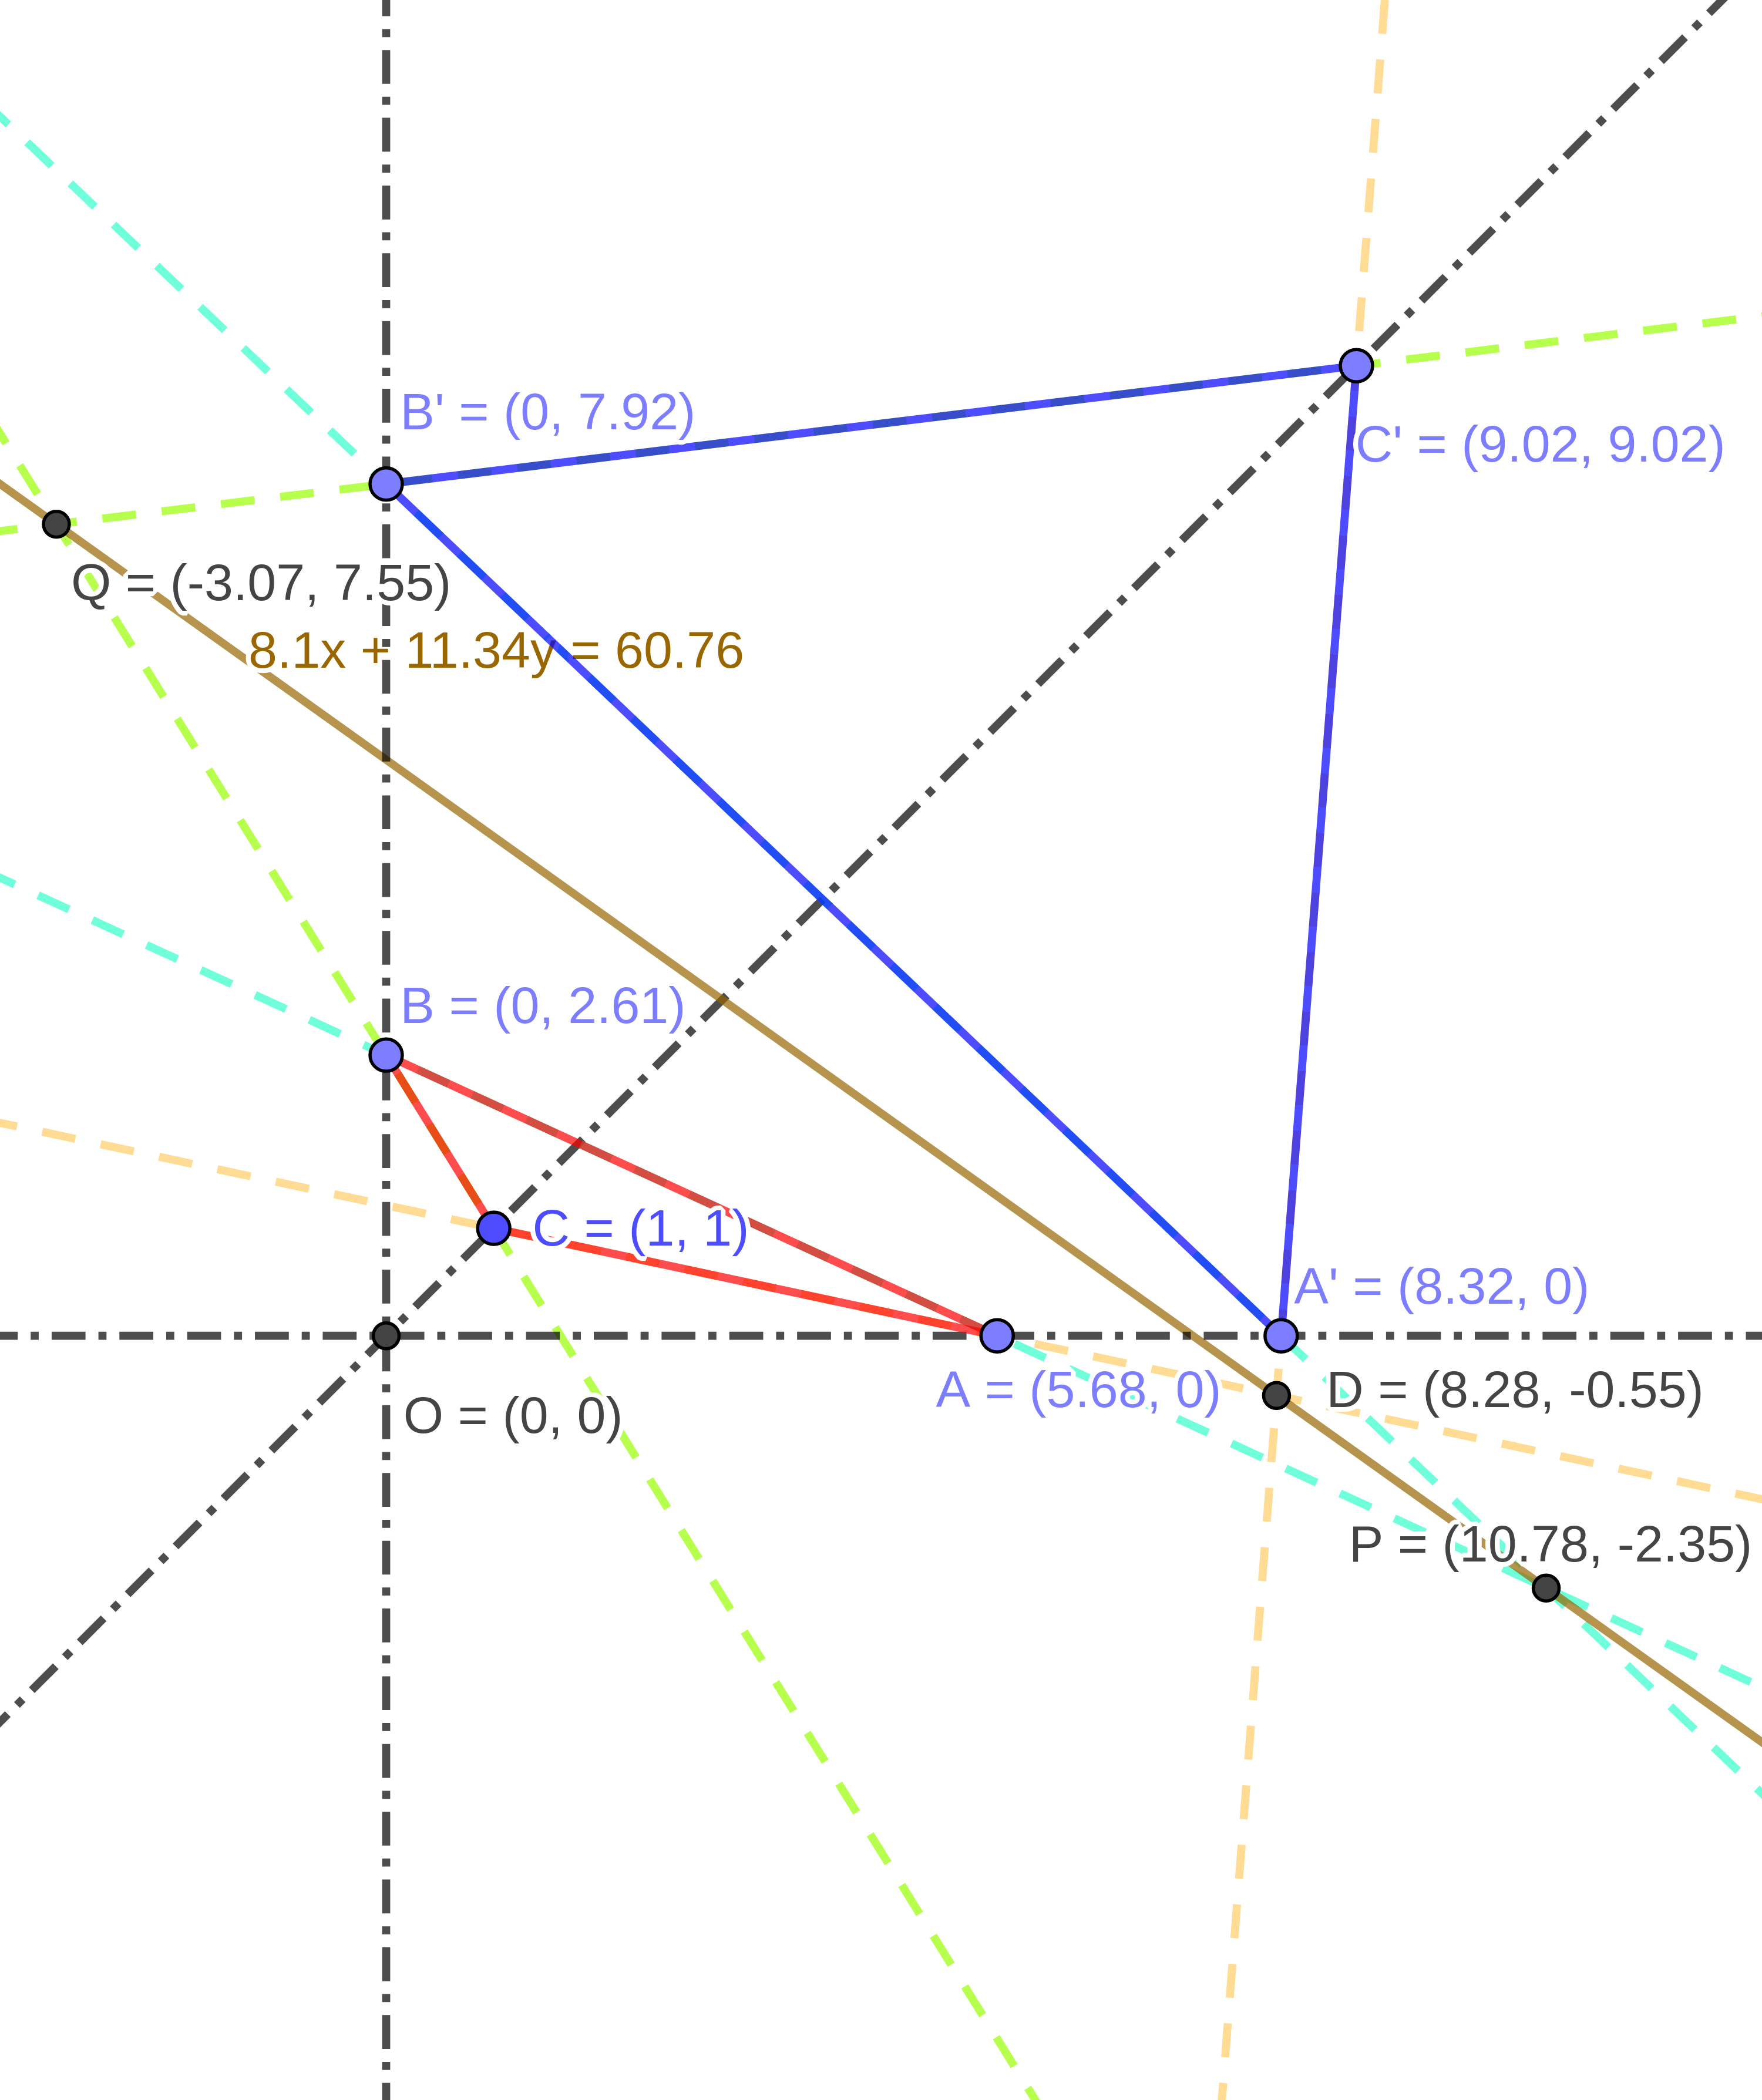
\includegraphics{Problema_02.png}
  \\
  Ejemplo del resultado obtenido.
  Imagen extra\'{\i}da del archivo Problema\_02(Desargues)(01).ggb
 \end{center}

\end{solucion}
